
\chapter{Analysis: Finding structure in Covariance}

We have seen in the Introduction that it can be useful to include difference in correlation into the distance of two distributions. In this section I will show a Proof of Concept and then apply the method to real-world data to show that in practice new insights are won by the inclusion of covariance into the analysis. While I first create synthetic data with a  Hierarchical gaussian Mixture Model to show a proof of conccetp, I will later analyse the Germen Federal Election 2017 as well as the European Values Study. 

\section{Synthetic Data}

I will define in the following what I call the Hierarchical Gaussian Mixture Model as a tool to understand Wasserstein t-SNE on snynthetic data before we apply the method to real world data. Since t-SNE is a cloustering method le's first define the clusters in our model, which the we aim to visualize with the method without providing the cluster membership of each datapoint. 

\subsection{Hierarchical Gaussian Mixture}

A Hierarchical Gaussian Mixture is defined by K classes, from which we have $N_k$ datapoints each. Each class is defined by a meana and Covariance matrix ...

\begin{figure}
	\centering
		\includegraphics[width=0.6\textwidth]{HGM/EasyHGM.pdf}
	\caption{Example of a HGM}
	\label{HGMclean}
\end{figure}

\subsection{Proof of Concept}

It is easy to image an example in which the information about the means is not enough to cluster the data, while a Wasserstein t-SNE approach succesgully does. In Figure \ref{HGMpoc} we can see a HGM that consists of 4 classes, two of which share the mean while two of them share the Scale matrix. The Euclidean embedding expectely doesn't cpature the structuire of the dataset, at the same time the sole information about Coavrarince isn't enough neither. The convex combination of both, the Wasserstein embedding, hoewver sepreates all 4 classes from ach other and can there be considered superioir to the other in this setting. 

\begin{figure}
	\centering
	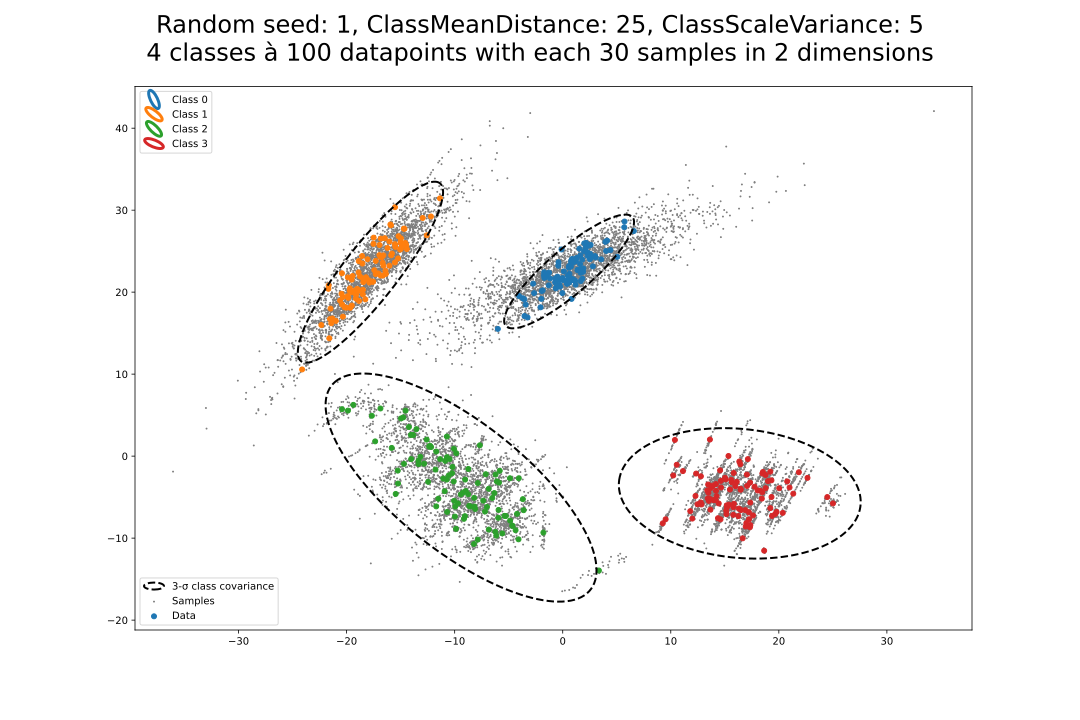
\includegraphics[width=1.1\textwidth]{HGM/CleanExample.pdf}
	\caption{Proof of Concept}
	\label{HGMpoc}
\end{figure}




\subsection{Distance of Covariances}

In section 2 I introduced the interpolation of Covariance and Mean distances. However it is not intuitive how much contribution each of the two different aspect of distance have, inparticular, how much impact a different Covarince has to the Wasserstein distance. In the follwoing experiment I sampled $N=100$ Covariance matrices from a Wishart distribution and computed the distance to a reference Covariance $\Sigma$ with the above described formula.  

We can see that 


\section{European Value Study 2017-2020}
\label{EVS}

So far we have been looking at synthetic data, \ie we designed the data in a way that they contain structure in the covariance and then showed, that the method is able to integrate this structure into the embedding. In this section however we want to find out, whether a real-world data set contains structure in the covariance. As a first example we analyse the European Values Study. It was collected in ... 

\subsection{Discrete Data}

In contrast to the synthetic data the EVS has discrete data, \ie each feature (question) is answered by a discrete value from 1 to 10. 

\begin{figure}
	\centering
	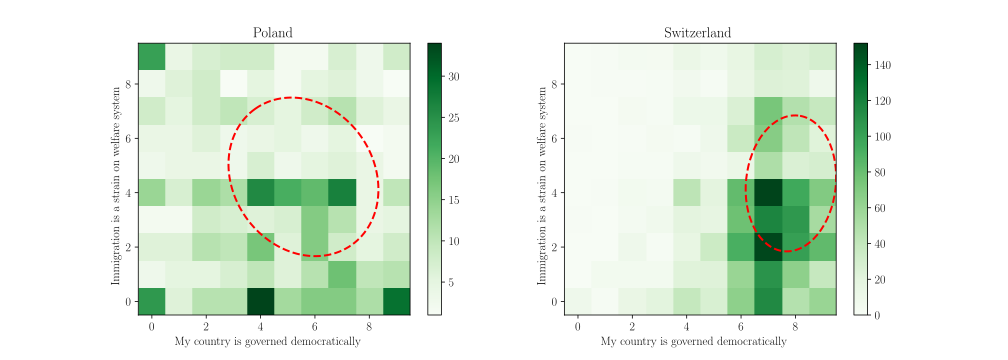
\includegraphics[width=1.1\textwidth]{EVS/Correlation_plchv143v187.pdf}
	\caption{Discrete Data}
	\label{EVSoverview}
\end{figure}

It it easy to see that the Gaussian approximation in Figure \ref{EVSVSoverview} is far from accurate, however we argue that it is still more accurate than taking only the mean. Also we will find in section \ref{WTevs} that the approximation leads to fair results compared to the Exact Wasserstein embedding. Later, in section \ref{GER} we will analyse a continuous dataset that perfectly fits the Gaussian approxmiation.

\subsection{Embeddings}

\begin{figure}
	\centering
	\includegraphics[width=\textwidth]{EVS/Embedding.pdf}
	\caption{Embedding}
	\label{EVSembedding}
\end{figure}

\begin{figure}
	\centering
	\includegraphics[width=\textwidth]{EVS/FeatureMeans.pdf}
	\caption{Features}
	\label{EVSfeatures}
\end{figure}

\subsection{Covariance}

\begin{figure}
	\centering
	\includegraphics[width=\textwidth]{EVS/Covariances.pdf}
	\caption{Covariance}
	\label{EVSembedding}
\end{figure}



\subsection{Comparison to Exact Wasserstein Embedding}
\label{WTevs}



\section{German Election 2017/2021}
\label{GER}

The Federal German Election is divided into 299 voting districts, each of which consists of roughly 150-850 poll stations (voting by mail excluded). In the following analysis we shall find that certain parties correlate differently within these voting districts, i.e. that

For simplification we exclude any party from the nalysis that hasn't received a minimum share of 5 per cent of the total votes. Otherwise the correlation would be manipulated by parties that only get elected in a specific state.


\subsection{Embeddings}

The plain Euclidean t-SNE embedding as well as the Pure Covariance embedding of the GER dataset are givven in Figure xy. In the middle we see the interlpolation of $\lambda = 0.75$. Interestingly the middle one has 4 clusters wheras the outer ones only admit 3 clusters. 



\subsubsection{Gaussian Wasserstein}

If we look at the legend in the appendix we see that the clusters share certain meta inforamtion: university cities, easetrn germany, southern Germany, western germany. 

\begin{figure}
	\centering
	\includegraphics[width=\textwidth]{GER/Embedding_small.pdf}
	\caption{GER embedding}
	\label{GERembed}
\end{figure}


\subsubsection{Exact Wasserstein}

\begin{figure}
	\centering
	\includegraphics[width=\textwidth]{GER/WassersteinComparison.pdf}
	\label{GERexact}
	\caption{GER correlation}
\end{figure}

\subsection{Covariance}


It is interesting to analyse if the structure in covariance is due to different correlations or mainly due to variance of each individual feature. In Figure xy we differentiate these two causes and observe that both factores play a role here. 

\begin{figure}
	\centering
	\includegraphics[width=\textwidth]{GER/Covariances.pdf}
	\label{GERcov}
	\caption{GER correlation}
\end{figure}



We can see that both correlation and variance play a role ..

We see three clusters 


\subsection{Correlation}

Wasserstein t-SNE is useful if and only if there is structure within the correlation of the dataset features. In FIgure \ref{GERcorr} we show, that for this particualr dsataset this clearly holds. One can see that certain features (e.g. AfD and SPD) correlate in some voting district, but anti-correlate in others. 

\begin{figure}
	\centering
	\includegraphics[width=\textwidth]{GER/Correlation.pdf}
	\label{GERcorr}
	\caption{GER correlation}
\end{figure}

If we inspect how the correlation exactly looks like we need to look at 

\begin{figure}
	\centering
	\includegraphics[width=\textwidth]{GER/JointCorrelation_LinksAfD.pdf}
	\label{GERjoint1}
	\caption{GER correlation}
\end{figure}

